\documentclass{standalone}
\usepackage{tikz}
\usetikzlibrary{patterns, positioning}
\usepackage[sfdefault]{ClearSans} %% option 'sfdefault' activates Clear Sans as the default text font
\usepackage[T1]{fontenc}

\begin{document}
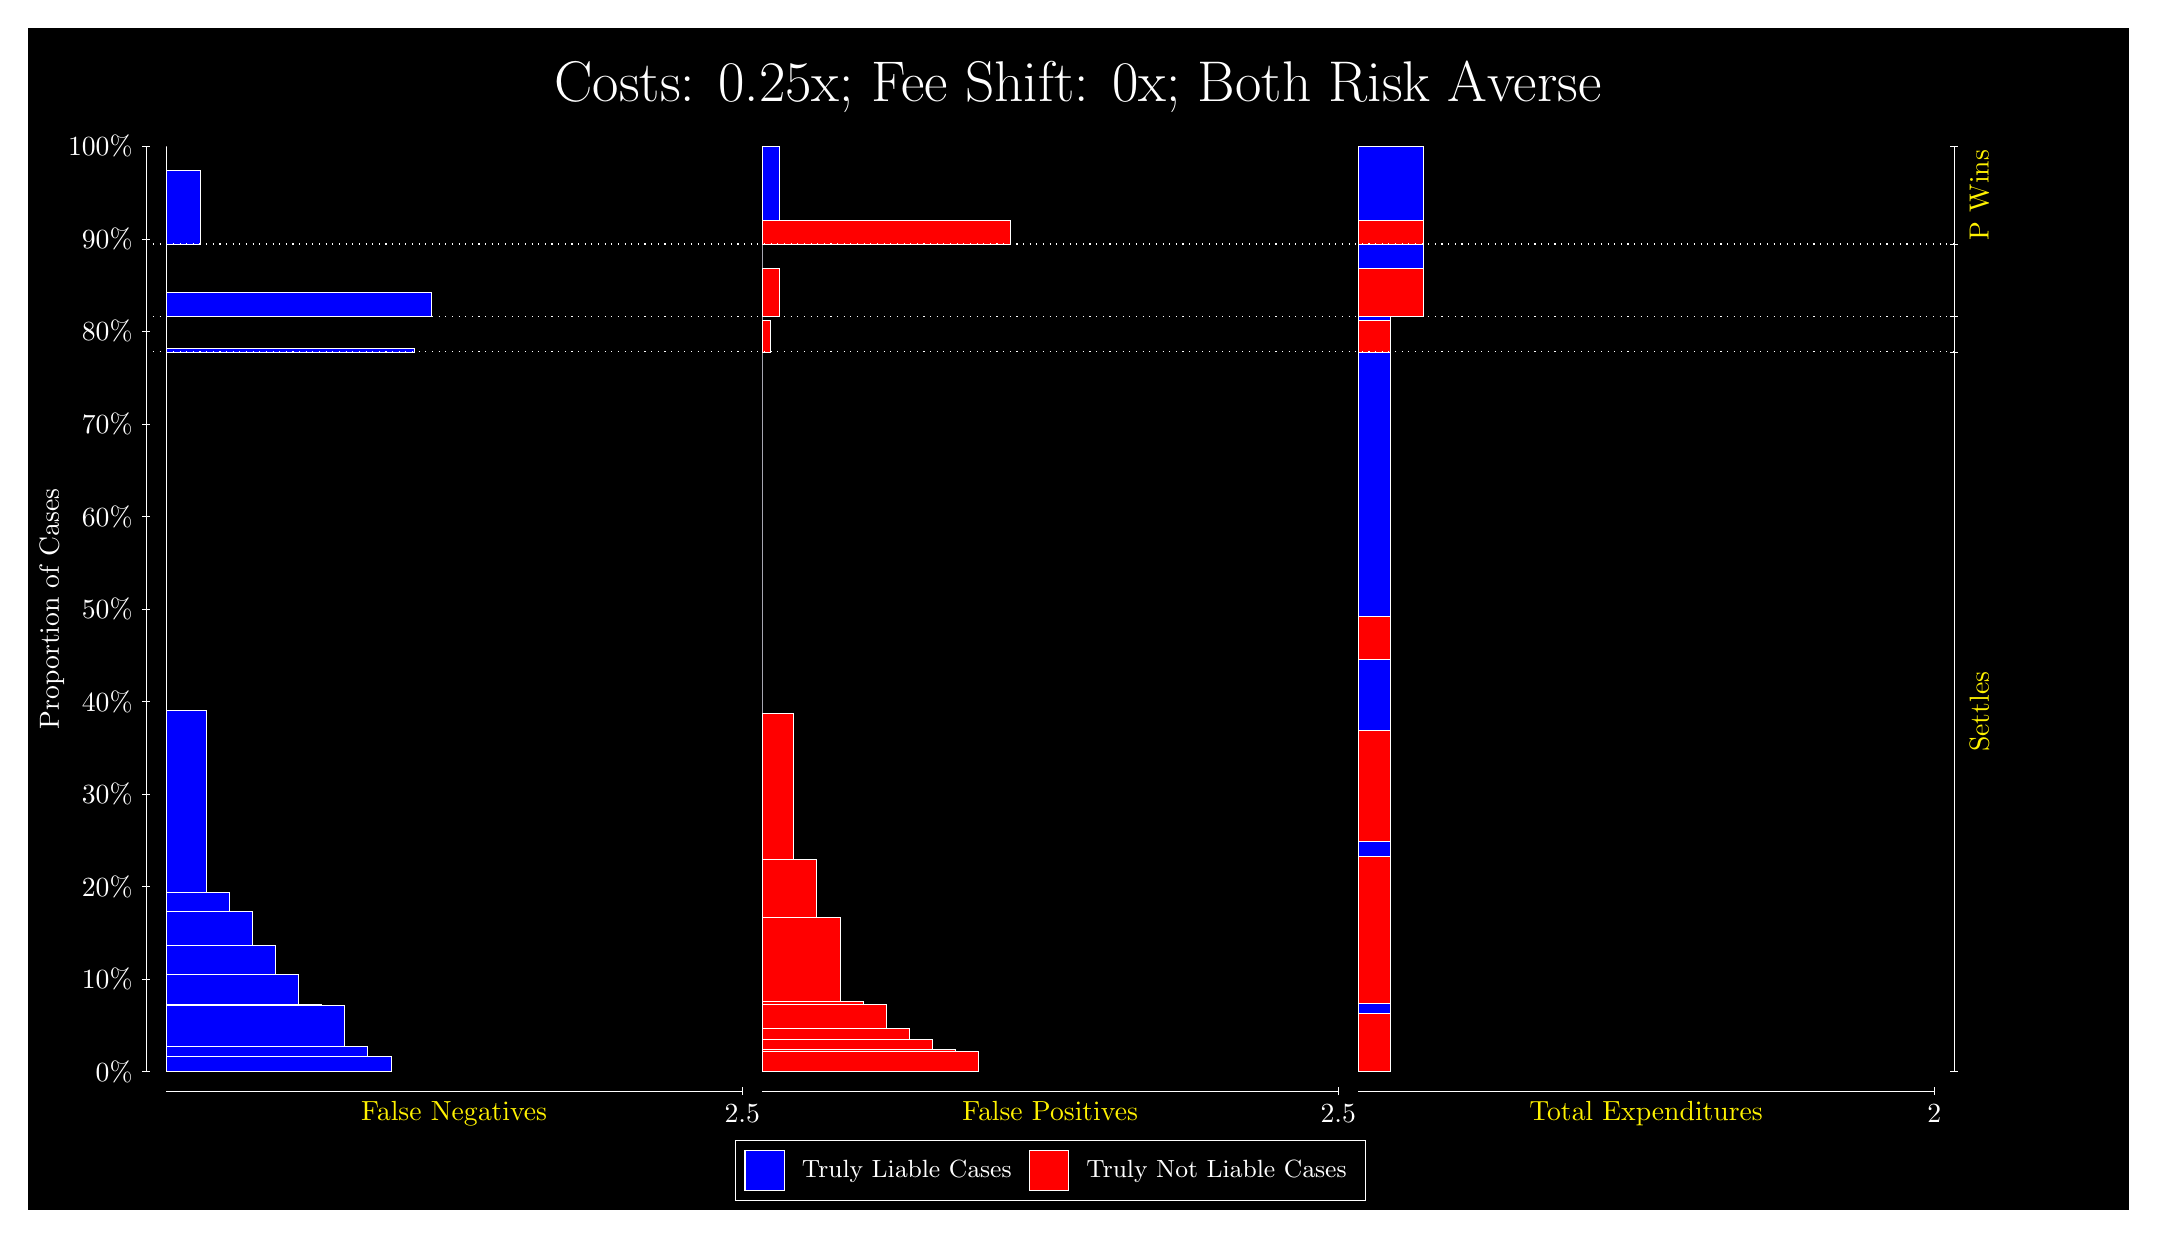
\begin{tikzpicture}
\draw[fill=black] (0,0) rectangle (26.667,15);
\draw[text=white] (0,13.5) rectangle (26.667,15) node[midway] {\huge Costs: 0.25x; Fee Shift: 0x; Both Risk Averse};
\draw[white, very thin] (1.5,1.75) -- (1.5,13.5);
\node[rotate=90, text=white, anchor=center] at (0.3, 7.625) {Proportion of Cases};
\draw[white, very thin] (1.45,1.75) -- (1.55,1.75);
\node[text=white, anchor=east] at (1.45, 1.75) {0\%};
\draw[white, very thin] (1.45,2.925) -- (1.55,2.925);
\node[text=white, anchor=east] at (1.45, 2.925) {10\%};
\draw[white, very thin] (1.45,4.1) -- (1.55,4.1);
\node[text=white, anchor=east] at (1.45, 4.1) {20\%};
\draw[white, very thin] (1.45,5.275) -- (1.55,5.275);
\node[text=white, anchor=east] at (1.45, 5.275) {30\%};
\draw[white, very thin] (1.45,6.45) -- (1.55,6.45);
\node[text=white, anchor=east] at (1.45, 6.45) {40\%};
\draw[white, very thin] (1.45,7.625) -- (1.55,7.625);
\node[text=white, anchor=east] at (1.45, 7.625) {50\%};
\draw[white, very thin] (1.45,8.8) -- (1.55,8.8);
\node[text=white, anchor=east] at (1.45, 8.8) {60\%};
\draw[white, very thin] (1.45,9.975) -- (1.55,9.975);
\node[text=white, anchor=east] at (1.45, 9.975) {70\%};
\draw[white, very thin] (1.45,11.15) -- (1.55,11.15);
\node[text=white, anchor=east] at (1.45, 11.15) {80\%};
\draw[white, very thin] (1.45,12.325) -- (1.55,12.325);
\node[text=white, anchor=east] at (1.45, 12.325) {90\%};
\draw[white, very thin] (1.45,13.5) -- (1.55,13.5);
\node[text=white, anchor=east] at (1.45, 13.5) {100\%};

\draw[white, very thin] (24.457,1.75) -- (24.457,13.5);
\draw[white, very thin] (24.407,1.75) -- (24.507,1.75);
\node[anchor=west] at (24.407, 1.75) {};
\draw[white, very thin] (24.407,10.89) -- (24.507,10.89);
\node[anchor=west] at (24.407, 10.89) {};
\draw[white, very thin] (24.407,11.34) -- (24.507,11.34);
\node[anchor=west] at (24.407, 11.34) {};
\draw[white, very thin] (24.407,12.259) -- (24.507,12.259);
\node[anchor=west] at (24.407, 12.259) {};
\draw[white, very thin] (24.407,13.5) -- (24.507,13.5);
\node[anchor=west] at (24.407, 13.5) {};

\draw[white, very thin, fill=blue] (1.75,1.75) rectangle (4.6044,1.9407);
\draw[white, very thin, fill=blue] (1.75,1.9407) rectangle (4.3116,2.0743);
\draw[white, very thin, fill=blue] (1.75,2.0743) rectangle (4.0188,2.5887);
\draw[white, very thin, fill=blue] (1.75,2.5887) rectangle (3.7261,2.6098);
\draw[white, very thin, fill=blue] (1.75,2.6098) rectangle (3.4333,2.9822);
\draw[white, very thin, fill=blue] (1.75,2.9822) rectangle (3.1406,3.3471);
\draw[white, very thin, fill=blue] (1.75,3.3471) rectangle (2.8478,3.7913);
\draw[white, very thin, fill=blue] (1.75,3.7913) rectangle (2.5551,4.0267);
\draw[white, very thin, fill=blue] (1.75,4.0267) rectangle (2.2623,6.3354);
\draw[white, very thin, fill=red] (1.75,6.3354) rectangle (1.75,10.89);
\draw[white, very thin, fill=blue] (1.75,10.89) rectangle (4.8971,10.94);
\draw[white, very thin, fill=red] (1.75,10.94) rectangle (1.75,11.34);
\draw[white, very thin, fill=blue] (1.75,11.34) rectangle (5.1167,11.642);
\draw[white, very thin, fill=red] (1.75,11.642) rectangle (1.75,12.259);
\draw[white, very thin, fill=blue] (1.75,12.259) rectangle (2.1891,13.197);
\draw[white, very thin, fill=red] (1.75,13.197) rectangle (1.75,13.5);
\draw[white, very thin, fill=red] (9.3189,1.75) rectangle (12.063,2.0094);
\draw[white, very thin, fill=red] (9.3189,2.0094) rectangle (11.771,2.0349);
\draw[white, very thin, fill=red] (9.3189,2.0349) rectangle (11.478,2.1585);
\draw[white, very thin, fill=red] (9.3189,2.1585) rectangle (11.185,2.2961);
\draw[white, very thin, fill=red] (9.3189,2.2961) rectangle (10.892,2.6046);
\draw[white, very thin, fill=red] (9.3189,2.6046) rectangle (10.6,2.6365);
\draw[white, very thin, fill=red] (9.3189,2.6365) rectangle (10.307,3.7048);
\draw[white, very thin, fill=red] (9.3189,3.7048) rectangle (10.014,4.4413);
\draw[white, very thin, fill=red] (9.3189,4.4413) rectangle (9.7214,6.3051);
\draw[white, very thin, fill=blue] (9.3189,6.3051) rectangle (9.3189,10.89);
\draw[white, very thin, fill=red] (9.3189,10.89) rectangle (9.4287,11.29);
\draw[white, very thin, fill=blue] (9.3189,11.29) rectangle (9.3189,11.34);
\draw[white, very thin, fill=red] (9.3189,11.34) rectangle (9.5384,11.957);
\draw[white, very thin, fill=blue] (9.3189,11.957) rectangle (9.3189,12.259);
\draw[white, very thin, fill=red] (9.3189,12.259) rectangle (12.466,12.562);
\draw[white, very thin, fill=blue] (9.3189,12.562) rectangle (9.5384,13.5);
\draw[white, very thin, fill=red] (16.888,1.75) rectangle (17.299,2.4865);
\draw[white, very thin, fill=blue] (16.888,2.4865) rectangle (17.299,2.62);
\draw[white, very thin, fill=red] (16.888,2.62) rectangle (17.299,4.4839);
\draw[white, very thin, fill=blue] (16.888,4.4839) rectangle (17.299,4.6746);
\draw[white, very thin, fill=red] (16.888,4.6746) rectangle (17.299,6.0834);
\draw[white, very thin, fill=blue] (16.888,6.0834) rectangle (17.299,6.9913);
\draw[white, very thin, fill=red] (16.888,6.9913) rectangle (17.299,7.5373);
\draw[white, very thin, fill=blue] (16.888,7.5373) rectangle (17.299,10.89);
\draw[white, very thin, fill=red] (16.888,10.89) rectangle (17.299,11.29);
\draw[white, very thin, fill=blue] (16.888,11.29) rectangle (17.299,11.34);
\draw[white, very thin, fill=red] (16.888,11.34) rectangle (17.711,11.957);
\draw[white, very thin, fill=blue] (16.888,11.957) rectangle (17.711,12.259);
\draw[white, very thin, fill=red] (16.888,12.259) rectangle (17.711,12.562);
\draw[white, very thin, fill=blue] (16.888,12.562) rectangle (17.711,13.5);
\draw[white, dotted] (1.5,10.89) -- (24.457,10.89);
\draw[white, dotted] (1.5,11.34) -- (24.457,11.34);
\draw[white, dotted] (1.5,12.259) -- (24.457,12.259);
\draw[white, very thin] (1.75,1.5) -- (9.0689,1.5);
\node[text=yellow, anchor=north] at (5.4094, 1.5) {False Negatives};
\draw[white, very thin] (9.0689,1.45) -- (9.0689,1.55);
\node[text=white, anchor=north] at (9.0689, 1.45) {2.5};

\draw[white, very thin] (9.3189,1.5) -- (16.638,1.5);
\node[text=yellow, anchor=north] at (12.978, 1.5) {False Positives};
\draw[white, very thin] (16.638,1.45) -- (16.638,1.55);
\node[text=white, anchor=north] at (16.638, 1.45) {2.5};

\draw[white, very thin] (16.888,1.5) -- (24.207,1.5);
\node[text=yellow, anchor=north] at (20.547, 1.5) {Total Expenditures};
\draw[white, very thin] (24.207,1.45) -- (24.207,1.55);
\node[text=white, anchor=north] at (24.207, 1.45) {2};

\node[text=yellow, centered, rotate=90] at (24.777, 6.3202) {Settles};


\node[text=yellow, centered, rotate=90] at (24.777, 12.879) {P Wins};

\draw (12.978300999999998,1.5) node[draw=none] (baseCoordinate) {};
\begin{scope}[align=center]
        \matrix[scale=0.5, draw=white, below=0.5cm of baseCoordinate, nodes={draw}, column sep=0.1cm]{
            \node[rectangle, draw, minimum width=0.5cm, minimum height=0.5cm, fill=blue] {}; &
            \node[draw=none, font=\small, text=white] (B) {Truly Liable Cases}; &
            \node[rectangle, draw, minimum width=0.5cm, minimum height=0.5cm, fill=red] {}; &
            \node[draw=none, font=\small, text=white] (B) {Truly Not Liable Cases}; \\
            };
\end{scope}

\end{tikzpicture}
\end{document}